% ==================================================================
% Prediction and validation --- includable fragment
% Numbers come from 06_prediction_validation.Rmd.
% ==================================================================

\providecommand{\TODO}[1]{\textbf{[TODO: #1]}}
\providecommand{\figplaceholder}[1]{%
  \framebox[0.8\textwidth]{%
    \parbox[c][4cm][c]{0.75\textwidth}{\centering\itshape #1}}}

% ------------------------------------------------------------------
\section{Prediction and validation}
\label{sec:prediction}
% ------------------------------------------------------------------
Everything up to this point has been estimated on the \num{1213}-customer
training subsample. This section confronts the model with the \num{128274}
held-out customers set aside in Section~\ref{sec:problem}, which were never
used for fitting, standardisation or variable selection. Following the
conclusion of Section~\ref{sec:sensitivity}, the horseshoe model is the one
carried forward here; the corresponding comparison against the vague-prior
logit and against BAS is reported in Appendix~\ref{app:bas_vs_hs}.

\subsection{From posterior draws to predicted probabilities}
For a held-out customer with covariate row $\tilde{x}_i$, the Bayesian point
prediction is the posterior mean of the success probability, obtained by
pushing every retained draw through the inverse link and averaging:
\begin{equation}
  \hat{p}_i \;=\;
  \frac{1}{S}\sum_{s=1}^{S}
  \operatorname{logit}^{-1}\!\Bigl(
      \beta_0^{(s)} + \tilde{x}_i^{\top}\beta^{(s)}
      + \beta_{\text{mid}}^{(s)}\,\texttt{midflight\_delay}_i
  \Bigr),
  \label{eq:postpred}
\end{equation}
This averages the transformed draws rather than transforming the averaged
ones: $\operatorname{logit}^{-1}$ is non-linear, so
$\mathbb{E}[g(\theta)] \neq g(\mathbb{E}[\theta])$, and only the former
propagates posterior uncertainty. Test covariates are standardised with the
\emph{training} means and standard deviations, so nothing from the held-out
set enters the fit.

\subsection{Discrimination and probabilistic accuracy}
We report two complementary summaries. The area under the ROC curve (AUC)
measures how well the model \emph{ranks} customers and is invariant to the
cutoff. The Brier score,
\begin{equation}
  \mathrm{BS} \;=\; \frac{1}{n}\sum_{i=1}^{n}\bigl(\hat{p}_i - y_i\bigr)^2 ,
  \label{eq:brier}
\end{equation}
is a strictly proper scoring rule, minimised only when the stated
probabilities match the true ones, so it rewards predictions that are both
well ranked and numerically honest. On the held-out set the horseshoe model
attains an AUC of $0.900$ and a Brier score of $0.126$.

\subsection{Classification and the choice of cutoff}
Turning probabilities into hard classifications requires a cutoff.
Table~\ref{tab:pred-cutoff} contrasts the conventional $0.5$ with the training
base rate $\bar{y} = 0.546$, the natural alternative when the two classes are
not perfectly balanced.

\begin{table}[htbp]
\centering
\small
\caption{Classification performance on the held-out set at two cutoffs.}
\label{tab:pred-cutoff}
\setlength{\tabcolsep}{4pt}
\begin{tabular}{lccc}
\toprule
Cutoff & Sensitivity & Specificity & Accuracy \\
\midrule
$t = 0.5$              & 0.837 & 0.812 & 0.826 \\
$t = \bar{y} = 0.546$  & 0.815 & 0.843 & 0.828 \\
\bottomrule
\end{tabular}
\end{table}

Moving to the base rate trades about two points of sensitivity for three of
specificity and leaves accuracy essentially unchanged ($0.826$ against
$0.828$). That near-indifference is informative: the errors are not
concentrated on one side, and accuracy alone is a blunt instrument for
choosing an operating point. The right cutoff depends on what the two mistakes
cost, which is Section~\ref{sec:pred-loss}.

\subsection{Calibration}
Neither AUC nor accuracy asks whether the predicted probabilities \emph{mean}
what they claim: among customers the model calls $70\%$ likely to be satisfied,
roughly $70\%$ should be. This matters as much as discrimination here, since
the posterior predictive probability is the object we report.
Table~\ref{tab:calibration} bins the held-out set into deciles of predicted
probability against the observed rate.


Calibration is good in the upper half: from the seventh decile up, predicted
and observed agree closely ($0.801$ against $0.819$, $0.896$ against $0.937$).
In the middle the model is mildly over-confident about dissatisfaction,
predicting $0.33$ and $0.49$ in deciles four and five where the observed rates
are $0.26$ and $0.43$, and the lowest two deciles reverse that. So the model
separates the classes well at the extremes, where most predictions live, and
is least trustworthy around $\hat{p} \approx 0.3$--$0.6$, where the evidence
genuinely is ambiguous.

\begin{table}[htbp]
\centering
\small
\caption{Calibration by decile of predicted probability.}
\label{tab:calibration}
\setlength{\tabcolsep}{4pt}
\begin{tabular}{cccc}
\toprule
Decile & Mean predicted & Observed rate & $n$ \\
\midrule
1  & 0.035 & 0.122 & \num{12828} \\
2  & 0.100 & 0.125 & \num{12827} \\
3  & 0.195 & 0.163 & \num{12827} \\
4  & 0.326 & 0.260 & \num{12828} \\
5  & 0.489 & 0.430 & \num{12827} \\
6  & 0.658 & 0.637 & \num{12827} \\
7  & 0.801 & 0.819 & \num{12828} \\
8  & 0.896 & 0.937 & \num{12827} \\
9  & 0.946 & 0.984 & \num{12827} \\
10 & 0.977 & 0.997 & \num{12828} \\
\bottomrule
\end{tabular}
\end{table}

\subsection{Posterior predictive check by subgroup}
\label{sec:pred-ppc}
The checks above compare point predictions against outcomes. A posterior
predictive check asks more: taking the fitted model seriously as a generative
description and simulating whole replicated datasets from it, do those
replications reproduce features of the real data the fit never targeted? For
each posterior draw we simulate outcomes for the entire held-out set and
recompute the satisfaction rate within each level of \texttt{Class},
\texttt{Customer Type} and \texttt{Type of Travel}, giving a posterior
predictive distribution per subgroup, shown in Figure~\ref{fig:ppc}, to
compare the observed rate against.

\begin{figure}[htbp]
\centering
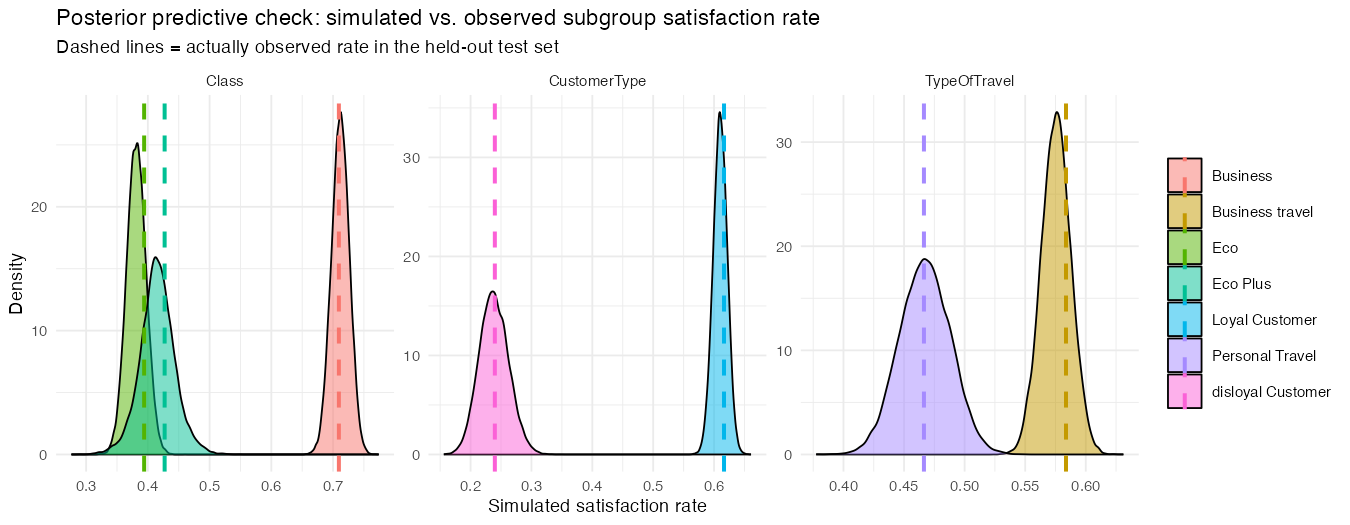
\includegraphics[width=0.75\linewidth]{img/prediction/ppc_subgroups.png}
\caption{Posterior predictive check by subgroup. Densities are the simulated
satisfaction rates; dashed lines mark the rates actually observed in the
held-out set.}
\label{fig:ppc}
\end{figure}

The observed rates fall inside the bulk of the simulated distributions for
every subgroup of all three variables, so the model is not systematically over-
or under-predicting satisfaction for any class of customer on data it has
never seen. The subgroup rates were never fitted directly, so reproducing them
is evidence that the covariate effects were captured rather than merely tuned
to the aggregate.

\subsection{Choosing the cutoff by expected loss}
\label{sec:pred-loss}
Rather than pick $0.5$ or the ROC-optimal point by convention, we state what
the two errors cost and minimise posterior expected loss. The airline flags a
customer when $\hat{p}_i < t$ and follows up with a retention contact; write
$C_{\text{miss}}$ for the cost of missing a dissatisfied customer and
$C_{\text{waste}}$ for that of contacting a satisfied one. The expected loss
at cutoff $t$ is
\begin{equation}
  \mathcal{L}(t) \;=\;
  C_{\text{miss}} \cdot \mathbb{P}\bigl(\hat{p} \ge t,\; y = 0\bigr)
  \;+\;
  C_{\text{waste}} \cdot \mathbb{P}\bigl(\hat{p} < t,\; y = 1\bigr),
  \label{eq:loss}
\end{equation}
estimated on the held-out set. Only the \emph{ratio} of the costs matters, so
the airline need not price either error, just say how many wasted contacts it
would trade for one retained customer. Table~\ref{tab:loss} gives the optimum
at three such ratios.

\begin{table}[htbp]
\centering
\small
\caption{Cutoff minimising expected loss, by assumed cost ratio
$C_{\text{miss}}\!:\!C_{\text{waste}}$.}
\label{tab:loss}
\setlength{\tabcolsep}{4pt}
\begin{tabular}{lcc}
\toprule
Cost ratio & Optimal cutoff $t^\star$ & Expected loss \\
\midrule
$1\!:\!1$ (equal cost) & 0.56 & 0.172 \\
$3\!:\!1$              & 0.74 & 0.252 \\
$5\!:\!1$              & 0.80 & 0.287 \\
\bottomrule
\end{tabular}
\end{table}

Under equal costs the optimum is $t^\star = 0.56$, essentially the base rate
and close to the conventional $0.5$, a useful sanity check on
Equation~\eqref{eq:loss}. As missing a dissatisfied customer grows more
expensive the cutoff rises, to $0.74$ at $3\!:\!1$ and $0.80$ at $5\!:\!1$: the
airline flags far more customers, accepting wasted contacts to catch the
recoverable ones. This is where the Bayesian machinery pays off operationally.
Because the model returns a calibrated distribution rather than a label, the
same fit supports any cost structure the business specifies, and the cutoff
follows from the loss function instead of convention.

% ==================================================================
\section{Conclusions}
\label{sec:conclusions}
% ==================================================================
We modelled airline customer satisfaction with a Bernoulli-logit likelihood,
first on the reduced covariate set suggested by the brief and then on the full
set under a horseshoe shrinkage prior, with \texttt{BAS} model averaging as an
independent cross-check. All posteriors were sampled by MCMC in JAGS.

Three effects dominate and survive every specification. Customer loyalty is the
strongest by a wide margin and the least shrunk coefficient at every global
scale tested; \emph{Inflight entertainment} and \emph{Business} class follow,
essentially tied ($\kappa_j = 0.17$ and $0.19$). Entertainment is the service
item the prior preserves most clearly, while \emph{Inflight wifi service} is
heavily shrunk despite correlating at $0.67$ with \emph{Online boarding} inside
the same booking cluster. That asymmetry is what the horseshoe was chosen for.

These conclusions are not artefacts of our modelling choices. The vague-prior
posterior moves by at most $0.066$ across four orders of magnitude of prior
variance; one predictor of twenty-two changes its signal/noise verdict across a
hundred-fold range of the global scale, and it sits on the $\kappa = 0.5$
boundary; and a training set twelve times larger moves the coefficients we
report by at most $0.022$. Out of sample, on \num{128274} unseen customers, the
model reaches an AUC of $0.900$, classifies $82.8\%$ correctly, and reproduces
the observed satisfaction rate in every subgroup.

One result resisted explanation: \emph{Departure/Arrival time convenient}
carries a negative coefficient whose interval excludes zero, and refitting
without the structural-zero rows strengthened it rather than weakening it, so
we report it as an open question. Three limitations are worth naming. The
structural zeros were flagged and tested but not modelled with a zero-inflated
likelihood; $n \approx 1200$ is modest for twenty-two predictors, which is why
several effects are borderline.
